\documentclass[a4paper,12pt]{article}

% Paquetes
\usepackage[utf8]{inputenc}
\usepackage{graphicx}
\usepackage{amsmath, amssymb}
\usepackage[margin = 1in]{geometry}
\usepackage[spanish, es-tabla]{babel}
\spanishdecimal{.}
\usepackage{color}
\usepackage{hyperref}

\usepackage{inconsolata}
\usepackage{listings}
\usepackage{xcolor}

\lstset{
    language=C,
    basicstyle=\ttfamily\scriptsize,
    numbers=left,
    numberstyle=\tiny,
    numbersep=5pt,
    %backgroudcolor={gray!10},
    keywordstyle=\color{blue},
    commentstyle=\color{gray},
    stringstyle=\color{red},
    showstringspaces=false,
    frame=single,
    breaklines=true,
    tabsize=2,
    captionpos=t,
    extendedchars=true,
    literate={á}{{\'a}}1 {é}{{\'e}}1 {í}{{\'i}}1 {ó}{{\'o}}1 {ú}{{\'u}}1 {Ú}{{\'U}}1 {ñ}{{\~{n}}}1 {°}{{$^{\circ}$}}1
}

% Comandos
\newcommand{\R}{\mathbb{R}}
\newcommand{\Z}{\mathbb{Z}}
\newcommand{\N}{\mathbb{N}}
\newcommand{\var}{\operatorname{Var}}
\newcommand{\E}{\mathbb{E}}
\newcommand{\norm}[1]{\left\Vert#1\right\Vert}

\renewcommand{\O}{\mathcal{O}}
\renewcommand{\P}{\mathbb{P}}

% Título
\title{Física computacional - Modelo de Ising \\ Laboratorio 4}
\author{El mono}
\date{}

% Documento
\begin{document}

\maketitle

\begin{abstract}
    Simulamos el modelo de Ising y calculamos algunas variables termodinámicas usando el método Metropolis. Estudiamos la dependencia de estas variables con respecto a la temperatura del sistema y, en particular, observamos que existe una temperatura crítica $T_c$ en la cual la magnetización presenta una bifurcación. Esto es, una transición de fase.
\end{abstract}

\section{Introducción}

Simulamos el modelo de Ising y calculamos algunas variables termodinámicas usando Markov Chain Monte Carlo (MCMC) con una cadena generada mediante el método Metropolis. Concretamente, simulamos un toro discreto de $n^2$ partículas, cada una de las cuales puede tener spin {\it up} o {\it down}; y calculamos, en función de la temperatura $T^*$ (adimensionalizada) la magnetización $M$, la energía $E$, la susceptibilidad $\chi$, el calor específico $C$ y la temperatúra crítica $T_c$. Estos cálculos son, en general, de la forma
\begin{equation}
    \label{eq:ejemplo}
    Q = \E(f_Q(X)),
\end{equation}
donde $X : \Omega \to S$ es una variable aleatoria que cae en el espacio $S$ de esatados del sistema con distribución de Boltzman, y $f_Q : S \to \R$ es alguna función por medio de la cual se calcula la cantidad $Q$. Dado que el espacio de estados es de cardinal $2^{n^2}$ (pues cada una de las $n^2$ partículas puede tener spin {\it up} o {\it down}), es demasiado costoso calcular $Q$ por definición. Por esta razón se opta, en general, por aproximar $Q$ mediante integración Monte Carlo (MC).\\

La integración MC para calcular \eqref{eq:ejemplo} requiere una forma de muestrear $X$, esto es, una forma de generar una sucesión de estados que sean realizaciones de varoiables $X_n$ independientes e idénticamente distribuídas con la distribución de $X$. Hay varias formas de hacer esto, una de ellas, mediante cadenas de Markov, se describe a continuación. Supongamos que existe una cadena de Markov $M = (M_n)$ sobre $S$ con una única distribución invariante $\pi$ igual a la distribución deseada (en este caso, la distribución de Boltzman). Entonces, independientemente de la distribución inicial (generalmente $M_0$ es uniforme o atómica), $M_n$ converge debilmente\footnote{Esto es, $\E(h(M_n)) \to \E(h(X))$ para toda $h$ continua y acotada.} a $X$. Así, a partir de cierto $N \in \N$, la cadena $\overline{M} = (M_{N + n})$ se distribuye aproximadamente $\pi$. El fragmento restante de la cadena: $M_0, M_1, \dots, M_{N - 1}$ se llama el {\it burn-in} y se descarta.

\newpage

Ahora, si bien $\overline{M}$ es un proceso de Markov donde cada $\overline{M}_n$ se distribuye aproximadamente $\pi$, los $\overline{M}_n$ podrían no ser independientes (recordemos que estamos en busca de una muestra de $X$, para lo cual la independencia es un factor crucial). En estas circunstancias es necesario extender la teoría de integración MC al caso MCMC con muestreo no independiente y calcular nuevamente la varianza de la integral. En este trabajo no discutimos estos cálculos, simplemente mencionamos que la varianza de la integral MC es ahora inversamente proporcional al número de muestras (como antes) y proporcional a $\tau_a$, una variable llamada tiempo de autocorrelación que representa, intuitivamente, cuantas muestras $\overline{M}_n$ debemos descartar para emular un muestreo independiente. En otras palabras, $\tau_a$ se define de forma que el proceso
\begin{equation*}
    \overline{\overline{M}} = (M_N, M_{N + \tau_a}, M_{N + 2\tau_a}, \dots)
\end{equation*}
no presente evidencia de dependencia.

Una forma ampliamente utilizada para construir una cadena de Markov con distribución invariante dada (en nuestro caso, la distribución de Boltzmann) es el método de Metropolis-Hastings. Este método define una cadena \( (M_n) \) sobre el espacio de estados \( S \) a partir de una \emph{propuesta} de transición, esto es, una familia de distribuciones de probabilidad \( g(x' \mid x) \), que especifica la probabilidad de proponer un nuevo estado \( x' \in S \) dado el estado actual \( x \in S \).\footnote{Formalmanete, se especifica una familia de medidas de probabilidad indexadas por $S$, pero por consistencia con la bibliografía estándar en el tema, denotamos esta familia por medio de sus funciones densidad condicional $g(\; \cdot \mid x)$ a pesar de que no necesariamente son absolutamente continuas con respecto a la medida de Lebesgue.} A partir del estado actual \( M_n = x \), se genera un candidato \( x' \sim g(\; \cdot \mid x) \), el cual es aceptado con probabilidad
\begin{equation}
    \label{eq:p_aceptacion}
    \P(\text{aceptar } x' \mid x) = \min \left\{1, \frac{\pi(x')\, g(x \mid x')}{\pi(x)\, g(x' \mid x)} \right\},
\end{equation}
y rechazado (manteniendo el estado actual \( M_{n+1} = x \)) con la probabilidad complementaria. Este procedimiento garantiza que la cadena resultante sea reversible con respecto a \( \pi \) y, bajo ciertas condiciones (que en nuestro caso se cumplen), ergódica. En particular, el método prouesto originalmente por Metropolis consideraba únicamente familias de distribuciones simétricas. Esto es, $g(x \mid x') = g(x' \mid x)$, de forma que la ecuación \eqref{eq:p_aceptacion} se simplifica.

\section{Resultados}

\begin{figure}
    \centering
    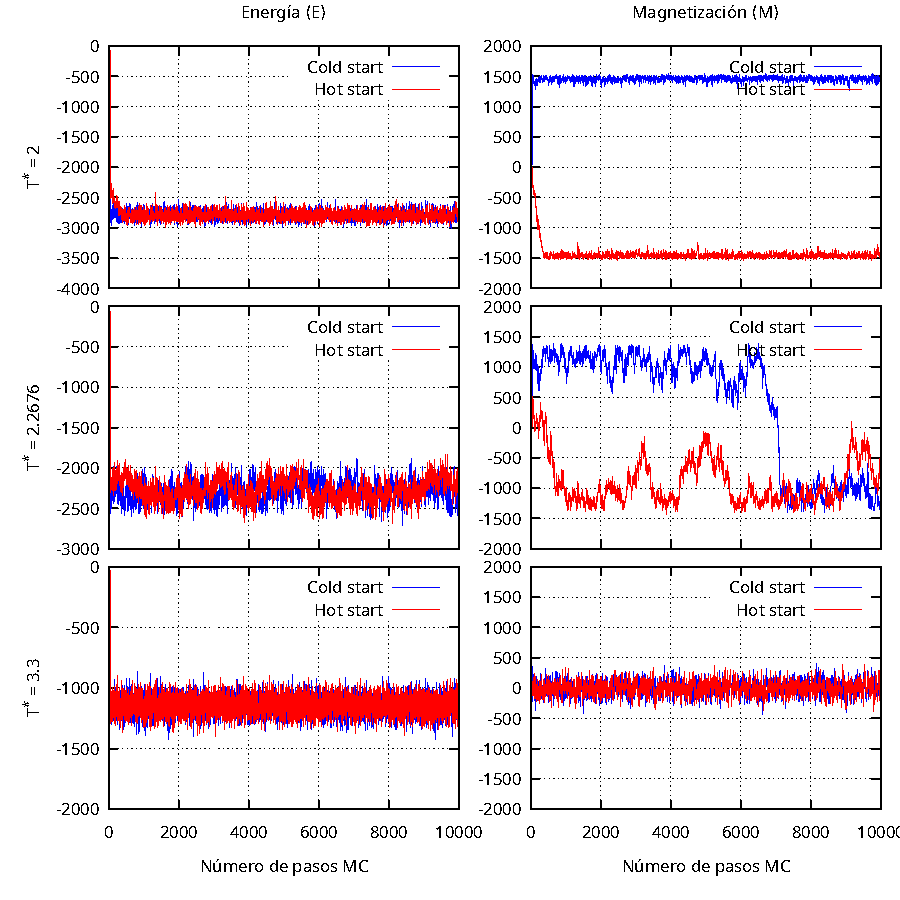
\includegraphics[width = \textwidth]{../img/a.pdf}
    \caption{Algún caption}
    \label{fig:a}
\end{figure}

\section{Discusión}

A medida que aumenta $n$, sabemos que la magnetización aleatoria se pelea con la temperatura. Si la temperatura $T^*$ es suficientemente grande, la probabilidad de aceptar un cambio crece, lo que conlleva mayor variabilidad de la magnetización en cada paso MC. Entonces, para temperaturas bajas, esperamos ver, en los {\it cold starts} que la magnetizacion general se mantiene, pues es poco propenso que el sistema acepte los cambios propuestos en un paso MC. Y en el {\it hot start}, esperamos ver uqe el sistema se decida rapidamente por una magnetización mas o menos uniforme y permanezca ahi. Esto es lo que se ve en los gráficos. Por mera casualidad, el hot start decidio estabilizarse con espin negativo...

Con respecto valores grandes de $T^*$ esperamos que la magnetización sea completamente aleatoria a lo largo de los pasos MC, pues se aceptan casi todos los cambios, sin importar si empezamos frios o calientes.

Lo interesante pasa para temperaturas intermedias. En $T^* = 2.2676$ observamos que la energía no se estabiliza, sinó que oscila (de forma no periódica) en un rango de enrgías. Al mismo tiempo, la magnetización tampoco se estabiliza, sinó que oscila entre períodos de magnetización casi uniformemente positiva y casi uniformemente negativa. Notemos ademas, que parecen coincidir los valores de $n$ para los cuales $\langle M \rangle$ oscila y $\langle E \rangle$ toma valores grandes. Esto nos indica que la distribución de Boltzman para este valor de $T^*$ es (hablando mal y pronto) bimodal, y la cadena de Markov del método de Metropolis debe pasar un tiempo en la región dominada por una de las modas y otro tiempo en la región dominada por la otra moda. A medida que la cadena transiciona entre ambas regiones, pasa por estados de energía mas alta, por esto las transiciones en $\langle M \rangle$ se corresponden con incrementos en $\langle E \rangle$.

Uno podría pensar que en este caso la integral MC no converge rápidamente, por lo que habría utilizar algún método alternativo, una cadena de Markov distinta quizas, o cualquier otra alternativa. Sin embargo, en la opinión del autor, el hecho de que $\langle M \rangle$ no converge es evidencia de que estamos haciendo la pregunta incorrecta, no de que somos incapaces de responderla. Me explico: si sabes que tu distribución es bimodal, qué sentido tiene preguntarte por la media? No es información representativa de la distribución. La integral MC calcula correctamente la media (si es cierto que tarda bastante mas en converger), pero preguntarse por la media en una bimodal es inútil. De hecho, en el caso $T^* = 0$ la distribución de Boltzman también es bimodal pero la integral de MC se estabiliza en una de las modas: ESTE ES EL VERDADERO ERROR! La verdadera integral de $M$ debería icluír información de ambas modas y equilibrarse en $\langle M \rangle = 0$. La falencia aquí es de la cadena de Markov del método de Metropolis, que no recorre correctamente el espacio de estados.

En principio, esto significa que no podemos confiar en los resultados calculados para temperaturas bajas! Sin embargo, dado que el sistema es simétrico con respecto al cambio de espines, aún podemos obtener resultados que ilustren el comportamiento del sistema si usamos el valor absoluto de la magnetización en lugar de la magnetización con signo. Repito: no cambiamos de $M$ a $|M|$ porque las cosas {\it se terminan promediando en 0} sino justamente porque no lo hacen. El problema es mas serio que simplemente no obtener información! ESTO TAMBIEN PODRÍA FRASEARSE COMO QUE ESTAMOS CAMBIANDO LA PREGUNTA.\\

Bueno, con respecto a los demas graficos no hay mucho que decir porque yo mismo no se mucho sober lo que esta pasando, puedo interpretar las probabilidades y demas cosas, pero no tanto la física. O decir a que corresponde macroscópicamente.... así que estas partes del informe van a quedar cortiñas... jaja willie cortiñas.

\section{Trabajo futuro}

ESTA ES LA ÚLTIMA SECCIÓN DE TRABAJO FUTURO, LA DEJO PARA TENER UNA REFERENCIA PARA ACTUALIZAR MAS TARDE.

Finalmente! Las imágenes tienen letra grande. Este es el más notorio de nuestros avances, pero hubo otros: adoptamos una estructura de carpetas {\it estandar} (en cierto sentido) para el código correspondiente a los ejercicios, automatizamos la compilación, testeo y generación de imágenes por medio de archivos \verb|makefile|, agregamos control de versiones por medio de Git y almacenamos el código en un repositorio online con GitHub. También estudiamos lo básico de CUDA, un lenguaje similar a C++ desarrollado por NVidia que permite programar para los procesadores de las GPUs, pero como los ejercicio de este laboratorio no eran demasiado costosos computacionalmente, no fue necesario implementar los generadores en este lenguaje. Esperamos, sin embargo, que cobre relevancia en laboratorios futuros.\\

Este ha sido, hasta el momento, el laboratorio más divertido. Entre las cosas que quedan por explorar, las más importantes son: el manual del compilador (opciones de optimización, tratar advertencias como errores, usar varios compiladores para detectar diferentes errores, etc), el lenguaje de scripting Bash, y temas básicos de mecánica estadística, para poder hacer los siguientes laboratorios.

%\section{Código}
%\label{sec:codice}
%\lstinputlisting[caption={Módulo con funciones auxiliares.}, label={lst:calor.c}]{../ej1/calor.c}

\bibliographystyle{abbrv}
\bibliography{biblio}

\end{document}